\section{Durchführung}
\label{sec:Durchführung}

Der Großteil dieses Versuches wird mit dem Programm XRD-Commander des Diffraktometers durchgeführt.
Zunächst wird dort der maximale Absorber eingeschaltet, damit die Intensität nicht zu hoch ist und Messgeräte beschädigt.
Die Probe wird an die entsprechnde Messposition gefahren.
Nun ist es möglich drei verschiedene Scans laufen zu lassen, einen Detektorscan, Z-Scan und Rockingscan.

Zunächst wird ein Detektor zur Justage durchgeführt.
Die Probe wird aus dem Strahl gefahren, in Z-Richtung, und die Röhre wird auf $\SI{0}{\degree}$ gestellt.
Der Detektor fährt nun einen kleinen Bereich, etwa $\SI{-0.5}{\degree}$ bis $\SI{0.5}{\degree}$, ab.
Die neue Nulllage des Detektors wird das Maximum der aufgenommenen Messung.

Die Probe wird wieder in den Strahl gefahren, nun wird die optimale Lage bestimmt, diese ist bei halber Abschattung der Intensität erreicht.
Dafür wird ein Z-Scan verwendet. 
Die Probe wird in Z-Richtung verschoben.
Aus den Messdaten wird die Position bei halber Intensität genommen und die Probe dorthin gefahren.

Danach folgt ein Rockingscan. 
Dabei wird die Röhre zusammen mit dem Detektor um die Probe gedreht, die Ausrichtig der beiden bleibt dabei gleich.
Die Funktionsweise eines Rockingscans ist in \autoref{fig:durch1} dargestellt.

\begin{figure}
    \centering
    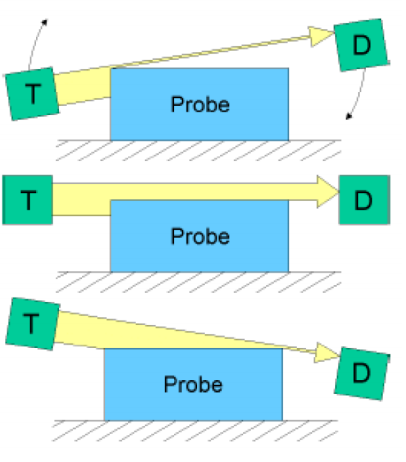
\includegraphics[width=0.5\textwidth]{images/rocking.png}
    \caption{Funktionsweise eines Rockingscans. \cite{V44}}
    \label{fig:durch1}
\end{figure}

Das Ergebnis sollte ein etwa symmetrisches Dreieick sein, falls das nicht der Fall ist muss in Y- Richtung nachjustiert werden.
Hier werden nun Röhre und Detektor zum Maximum der Verteilung bewegt.
Anschließend wird ein weiterer Z-Scan durchgeführt, wie oben bereits beschrieben.

Es wird ebenfalls ein weiterer Rockingscan dufchgeführt, allerdings stehen sich Röhre und Detektor hier nicht mehr direkt gegenüber. 
Nun werden allerdings Einfalls- und Ausfallswinkel auf $\SI{0.15}{\degree}$ gestellt.
Ansonsten wird wie oben verfahren. 
Es wird ebenfalls wieder ein Z-Scan durchgeführt.
Hier soll wieder die Position der halben Abschattung bestimmt werden, das Prinzip dieses Scanns ist in \autoref{fig:durch2} gezeigt.

\begin{figure}
    \centering
    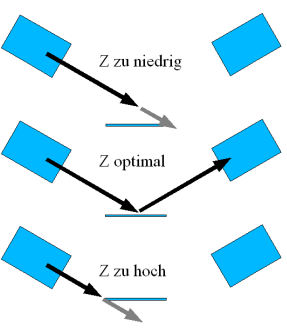
\includegraphics[width=0.5\textwidth]{images/z.png}
    \caption{Funktionsweise eines Z-Scans unter einem Winkel von $2 \theta = \SI{0.30}{\degree}$. \cite{V44}}
    \label{fig:durch2}
\end{figure}

Schlussendlich findet die eigentliche Messung statt.
Der Scantype wird auf Omega/2Theta gestellt und ein Scanbereich von $\SI{0}{\degree}$ bis $\SI{2.5}{\degree}$ eingestellt.
Die Schrittweite soll $\SI{0.005}{\degree}$ betragen bei einer Scanzeit von $\SI{5}{\second}$.
Anschließend wird die Messung erneut durchgeführt, allerdings wird Detektor um $\SI{0.1}{\degree}$ gegenüber der Röntgenröhre verschoben.
Dies ist der sogenannte Diffuse Scan und ist für die Auswertung des Versuch von großer Bedeutung.
Alle Ergebnisse dieses Experiments werden in .raw Datein gespeichert, damit die Plots für die Auswertung einsehbar sind.
